\documentclass[11pt,professionalfonts,hyperref={pdftex,pdfpagemode=none,pdfstartview=FitH}]{beamer}
%\usepackage{times}
%\usefonttheme{serif}
%\usepackage{helvet}
%\usepackage{amsmath,amssymb}
\usepackage{graphicx,multirow}
\usepackage[scriptsize]{subfigure}
%\usepackage{movie15}

%\usepackage{warmread}
%\usepackage[all,import]{xy}

%\renewcommand\mathfamilydefault{\rmdefault}

\newcommand{\norm}[1]{\ensuremath{\left\| #1 \right\|}}
\newcommand{\bracket}[1]{\ensuremath{\left[ #1 \right]}}
\newcommand{\braces}[1]{\ensuremath{\left\{ #1 \right\}}}
\newcommand{\parenth}[1]{\ensuremath{\left( #1 \right)}}
\newcommand{\pair}[1]{\ensuremath{\langle #1 \rangle}}
\newcommand{\met}[1]{\ensuremath{\langle\langle #1 \rangle\rangle}}
\newcommand{\refeqn}[1]{(\ref{eqn:#1})}
\newcommand{\reffig}[1]{Fig. \ref{fig:#1}}
\newcommand{\tr}[1]{\mathrm{tr}\ensuremath{\negthickspace\bracket{#1}}}
\newcommand{\trs}[1]{\mathrm{tr}\ensuremath{[#1]}}
\newcommand{\deriv}[2]{\ensuremath{\frac{\partial #1}{\partial #2}}}
\newcommand{\SO}{\ensuremath{\mathsf{SO(3)}}}
\newcommand{\T}{\ensuremath{\mathsf{T}}}
\renewcommand{\L}{\ensuremath{\mathsf{L}}}
\newcommand{\so}{\ensuremath{\mathfrak{so}(3)}}
\newcommand{\SE}{\ensuremath{\mathsf{SE(3)}}}
\newcommand{\se}{\ensuremath{\mathfrak{se}(3)}}
\renewcommand{\Re}{\ensuremath{\mathbb{R}}}
\newcommand{\aSE}[2]{\ensuremath{\begin{bmatrix}#1&#2\\0&1\end{bmatrix}}}
\newcommand{\ase}[2]{\ensuremath{\begin{bmatrix}#1&#2\\0&0\end{bmatrix}}}
\newcommand{\D}{\ensuremath{\mathbf{D}}}
\newcommand{\Sph}{\ensuremath{\mathsf{S}}}
\renewcommand{\S}{\Sph}
\newcommand{\J}{\ensuremath{\mathbf{J}}}
\newcommand{\Ad}{\ensuremath{\mathrm{Ad}}}
\newcommand{\intp}{\ensuremath{\mathbf{i}}}
\newcommand{\extd}{\ensuremath{\mathbf{d}}}
\newcommand{\hor}{\ensuremath{\mathrm{hor}}}
\newcommand{\ver}{\ensuremath{\mathrm{ver}}}
\newcommand{\dyn}{\ensuremath{\mathrm{dyn}}}
\newcommand{\geo}{\ensuremath{\mathrm{geo}}}
\newcommand{\Q}{\ensuremath{\mathsf{Q}}}
\newcommand{\G}{\ensuremath{\mathsf{G}}}
\newcommand{\g}{\ensuremath{\mathfrak{g}}}
\newcommand{\Hess}{\ensuremath{\mathrm{Hess}}}
\newcommand{\refprop}[1]{Proposition \ref{prop:#1}}

\definecolor{mygray}{gray}{0.9}

\mode<presentation> {
  \usetheme{Warsaw}
  \usefonttheme{serif}
  \setbeamercovered{transparent}
}

\newcommand{\mypaper}{}

\setbeamertemplate{footline}%{split theme}
{%
  \leavevmode%
  \hbox{\begin{beamercolorbox}[wd=.7\paperwidth,ht=2.5ex,dp=1.125ex,leftskip=.3cm,rightskip=.3cm plus1fill]{author in head/foot}%
    \usebeamerfont{author in head/foot}\insertshorttitle
  \end{beamercolorbox}%
  \begin{beamercolorbox}[wd=.5\paperwidth,ht=2.5ex,dp=1.125ex,leftskip=.3cm,rightskip=.3cm]{title in head/foot}
%    \usebeamerfont{title in head/foot}\mypaper\hfill \insertframenumber/\inserttotalframenumber
    \usebeamerfont{title in head/foot}\hfill \insertframenumber/\inserttotalframenumber
  \end{beamercolorbox}}%
  \vskip0pt%
} \setbeamercolor{box}{fg=black,bg=yellow}

\title[Bayesian Occupancy Grid Mapping via an Exact Inverse Sensor Model ]{\large Bayesian Occupancy Grid Mapping via an Exact Inverse Sensor Model}

\author{\vspace*{-0.3cm}}

\institute{\footnotesize
{\normalsize Evan Kaufman, Taeyoung Lee, \\Zhuming Ai, and Ira S. Moskowitz}\vspace*{0.2cm}\\
  Mechanical and Aerospace Engineering\\ George Washington University}

\date{}

\definecolor{tmp}{rgb}{0.804,0.941,1.0}
\setbeamercolor{numerical}{fg=black,bg=tmp}
\setbeamercolor{exact}{fg=black,bg=red}

\newtheorem{prop}{Proposition}



\renewcommand{\emph}[1]{\textit{\textbf{\color{blue}{#1}}}}


\begin{document}

\begin{frame}
  \titlepage
\end{frame}


\section*{}
\subsection*{Introduction}

\begin{frame}
\frametitle{Introduction}
\begin{itemize}
    \item Robotic Mapping
    \begin{itemize}
    	\item Goal: generate a map representing surrounding regions
	\item Crucial for simulataneous localization and mapping (SLAM) and autonomous exploration of uncertain environments
    	\item Popular mapping representations include occupancy grids, octomaps, and feature-based maps
    \end{itemize}
\item Occupancy Grid Mapping
\begin{itemize}
	\item The environment may be decomposed into evenly spaced grid cells that are either \emph{occupied} or \emph{free}
	\item Probabilistic map: the goal is to obtain the  probability of each grid cell being occupied
\end{itemize}
\end{itemize}

\only<1->{
\begin{figure}
\centerline{
    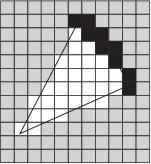
\includegraphics[height=2.1cm]{ogm_ex1.jpg}\hspace*{0.1cm}
\hspace*{0.5cm}
    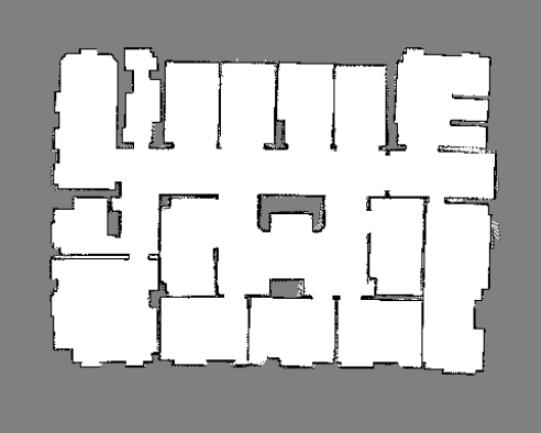
\includegraphics[height=2.1cm]{ogm_ex2.png}\hspace*{0.1cm}
\hspace*{0.5cm}
    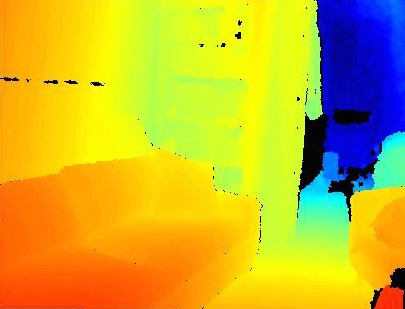
\includegraphics[height=2.1cm]{ogm_ex3.jpeg}\hspace*{0.1cm}
}
\end{figure}}

\end{frame}


\begin{frame}
\frametitle{Introduction}
\framesubtitle{Problem Definition}

\begin{itemize}
	\item The Map and the Robot
	\begin{itemize}
	\item Map $m$ is composed of $n_m$ grid cells
	\item The $i$-th grid cell $\mathbf{m}_i$ is a \emph{binary} random variable, independent of other grid cells: $P(m)=P(\mathbf{m}_1,\mathbf{m}_2,\ldots,\mathbf{m}_{n_m})=\prod_{i=1}^{n_m}P(\mathbf{m}_i)$
	\item The robot \emph{pose} $X_t$ contains the \emph{position} and \emph{attitude} of the robot at the $t$-th timestep, and the history of poses $X_{1:t}$ is known	
	\end{itemize}
\vspace*{0.3cm}\pause
	\item Depth Measurements
	\begin{itemize}
	\item The measurement origins and directions are known \emph{deterministically}
	\item A measurement \emph{scan} $Z_t=\braces{z_{t,1},z_{t,2},\ldots,z_{t,n_z}}$ contains $n_z$ measurement \emph{rays} (depth readings) at the $t$-th time step, and the history of measurement scans $Z_{1:t}$ is known
	\item The \emph{forward sensor model} is the probability density distribution $p(z_{t,l}|m,X_{t})$  known from the sensor properties
	\end{itemize}
\end{itemize}

\end{frame}

\begin{frame}
\frametitle{Introduction}
\framesubtitle{Problem Definition}

\begin{itemize}
	\item Bayesian Framework
	\begin{itemize}
	\item Markov Assumption
	\item Benefit of Log-Odds
	\item Assumption with Log-Odds
	\end{itemize}
\vspace*{0.3cm}\pause
	\item Inverse Sensor Model
	\begin{itemize}
	\item Equation
	\item Computationally intractable equation
	\item Motivation for another solution...
	\end{itemize}
\end{itemize}

\end{frame}

\begin{frame}
\frametitle{Introduction}
\framesubtitle{Problem Definition}

\begin{itemize}
	\item Heuristic Approach
	\begin{itemize}
	\item Idea
	\item Figure
	\item Mathematically innacurate
	\end{itemize}
\vspace*{0.3cm}\pause
	\item Learning
	\begin{itemize}
	\item Idea
	\item Complicated, not clear how parameters are chosen
	\end{itemize}
\vspace*{0.3cm}\pause
	\item Goal: design a simple and accurate method for occupancy grid mapping that avoids log-odds ratio assumptions
\end{itemize}

\end{frame}



\section*{}
\subsection*{Problem Formulation}


\begin{frame}
\frametitle{Single Measurement Ray}

\begin{itemize}
    \item Main idea: make use of occupancy grid mapping \emph{assumptions} and extract \emph{paterns} from probabilistic properties to find a \emph{computationally-efficient} solution
	\begin{itemize}
		\item Since the origin and direction of each measurement ray is known deterministically, the set of grid cells that the ray intersects is known through geometry
		\item A depth reading follows the forward sensor model, which \emph{only depends} on the first occupied grid cell along the measurement ray
		\item (figure on forward sensor model)
	\end{itemize}
\end{itemize}
\end{frame}

\begin{frame}
\frametitle{Single Measurement Ray}

\begin{itemize}
    \item Patterns...
	\begin{itemize}
		\item 
	\end{itemize}
\end{itemize}
\end{frame}




\begin{frame}
\frametitle{Full Measurement Scan}

\begin{itemize}
	\item 
\end{itemize}

\end{frame}


\section*{}
\subsection*{Results}

\begin{frame}
\frametitle{Numerical Example}

\begin{itemize}
\item 1D Case
\end{itemize}

\end{frame}

\begin{frame}
\frametitle{Numerical Example}

\begin{itemize}
\item 2D Case
\end{itemize}

\end{frame}


\begin{frame}
\frametitle{Experiment}

\begin{itemize}
\item Kinect
\end{itemize}

\end{frame}



\section*{}
\subsection*{Conclusions}

\begin{frame}
\frametitle{Conclusions}
\begin{itemize}
    \item 
    \begin{itemize}
        \item 
    \end{itemize}
\end{itemize}
\end{frame}



\end{document}

